\subsection{Models}

The train set used for this phase of exploring various classifiers consists of four main components: unigrams and bigrams, embeddings, stylistic features, and the offensiveness score. Depending on which embeddings dataset is used, the dimensionality may change, but it generally consists of approximately 7,000 total features.
{}

After tuning the hyperparameters of several classifiers (\textbf{Logistic Regression}, \textbf{SVM}, \textbf{Random Forest}, \textbf{XGBoost}, \textbf{Light-GBM}), \textbf{Light-GBM} emerged as the best performer, achieving an average F1-macro of 0.774 on 5 folds of cross-validation. Moreover, it proved to be the fastest. Thus, we employed this first version of the model to carry out several feature-focused analyses.

For instance, with respect to feature importance: although any of the four datasets manages, taken individually for training, to yield an average F1-macro of at least 0.75, the classification model primarily relies on the embeddings when all datasets are combined. It also considers a few other interesting features, such as the unigrams 'rom' and 'terrorism', the stylistic features 'uppercase\_words\_dist' and 'lexical\_density', as well as 'offensiveness\_score' and 'badword'.

Moreover, the calculation of feature importance revealed that the model does not benefit at all from many of our features, as it achieves its highest result (average F1-macro of 0.784) using only the first 100, as shown by the plot in Figure \ref{fig:features}.

\begin{figure}
    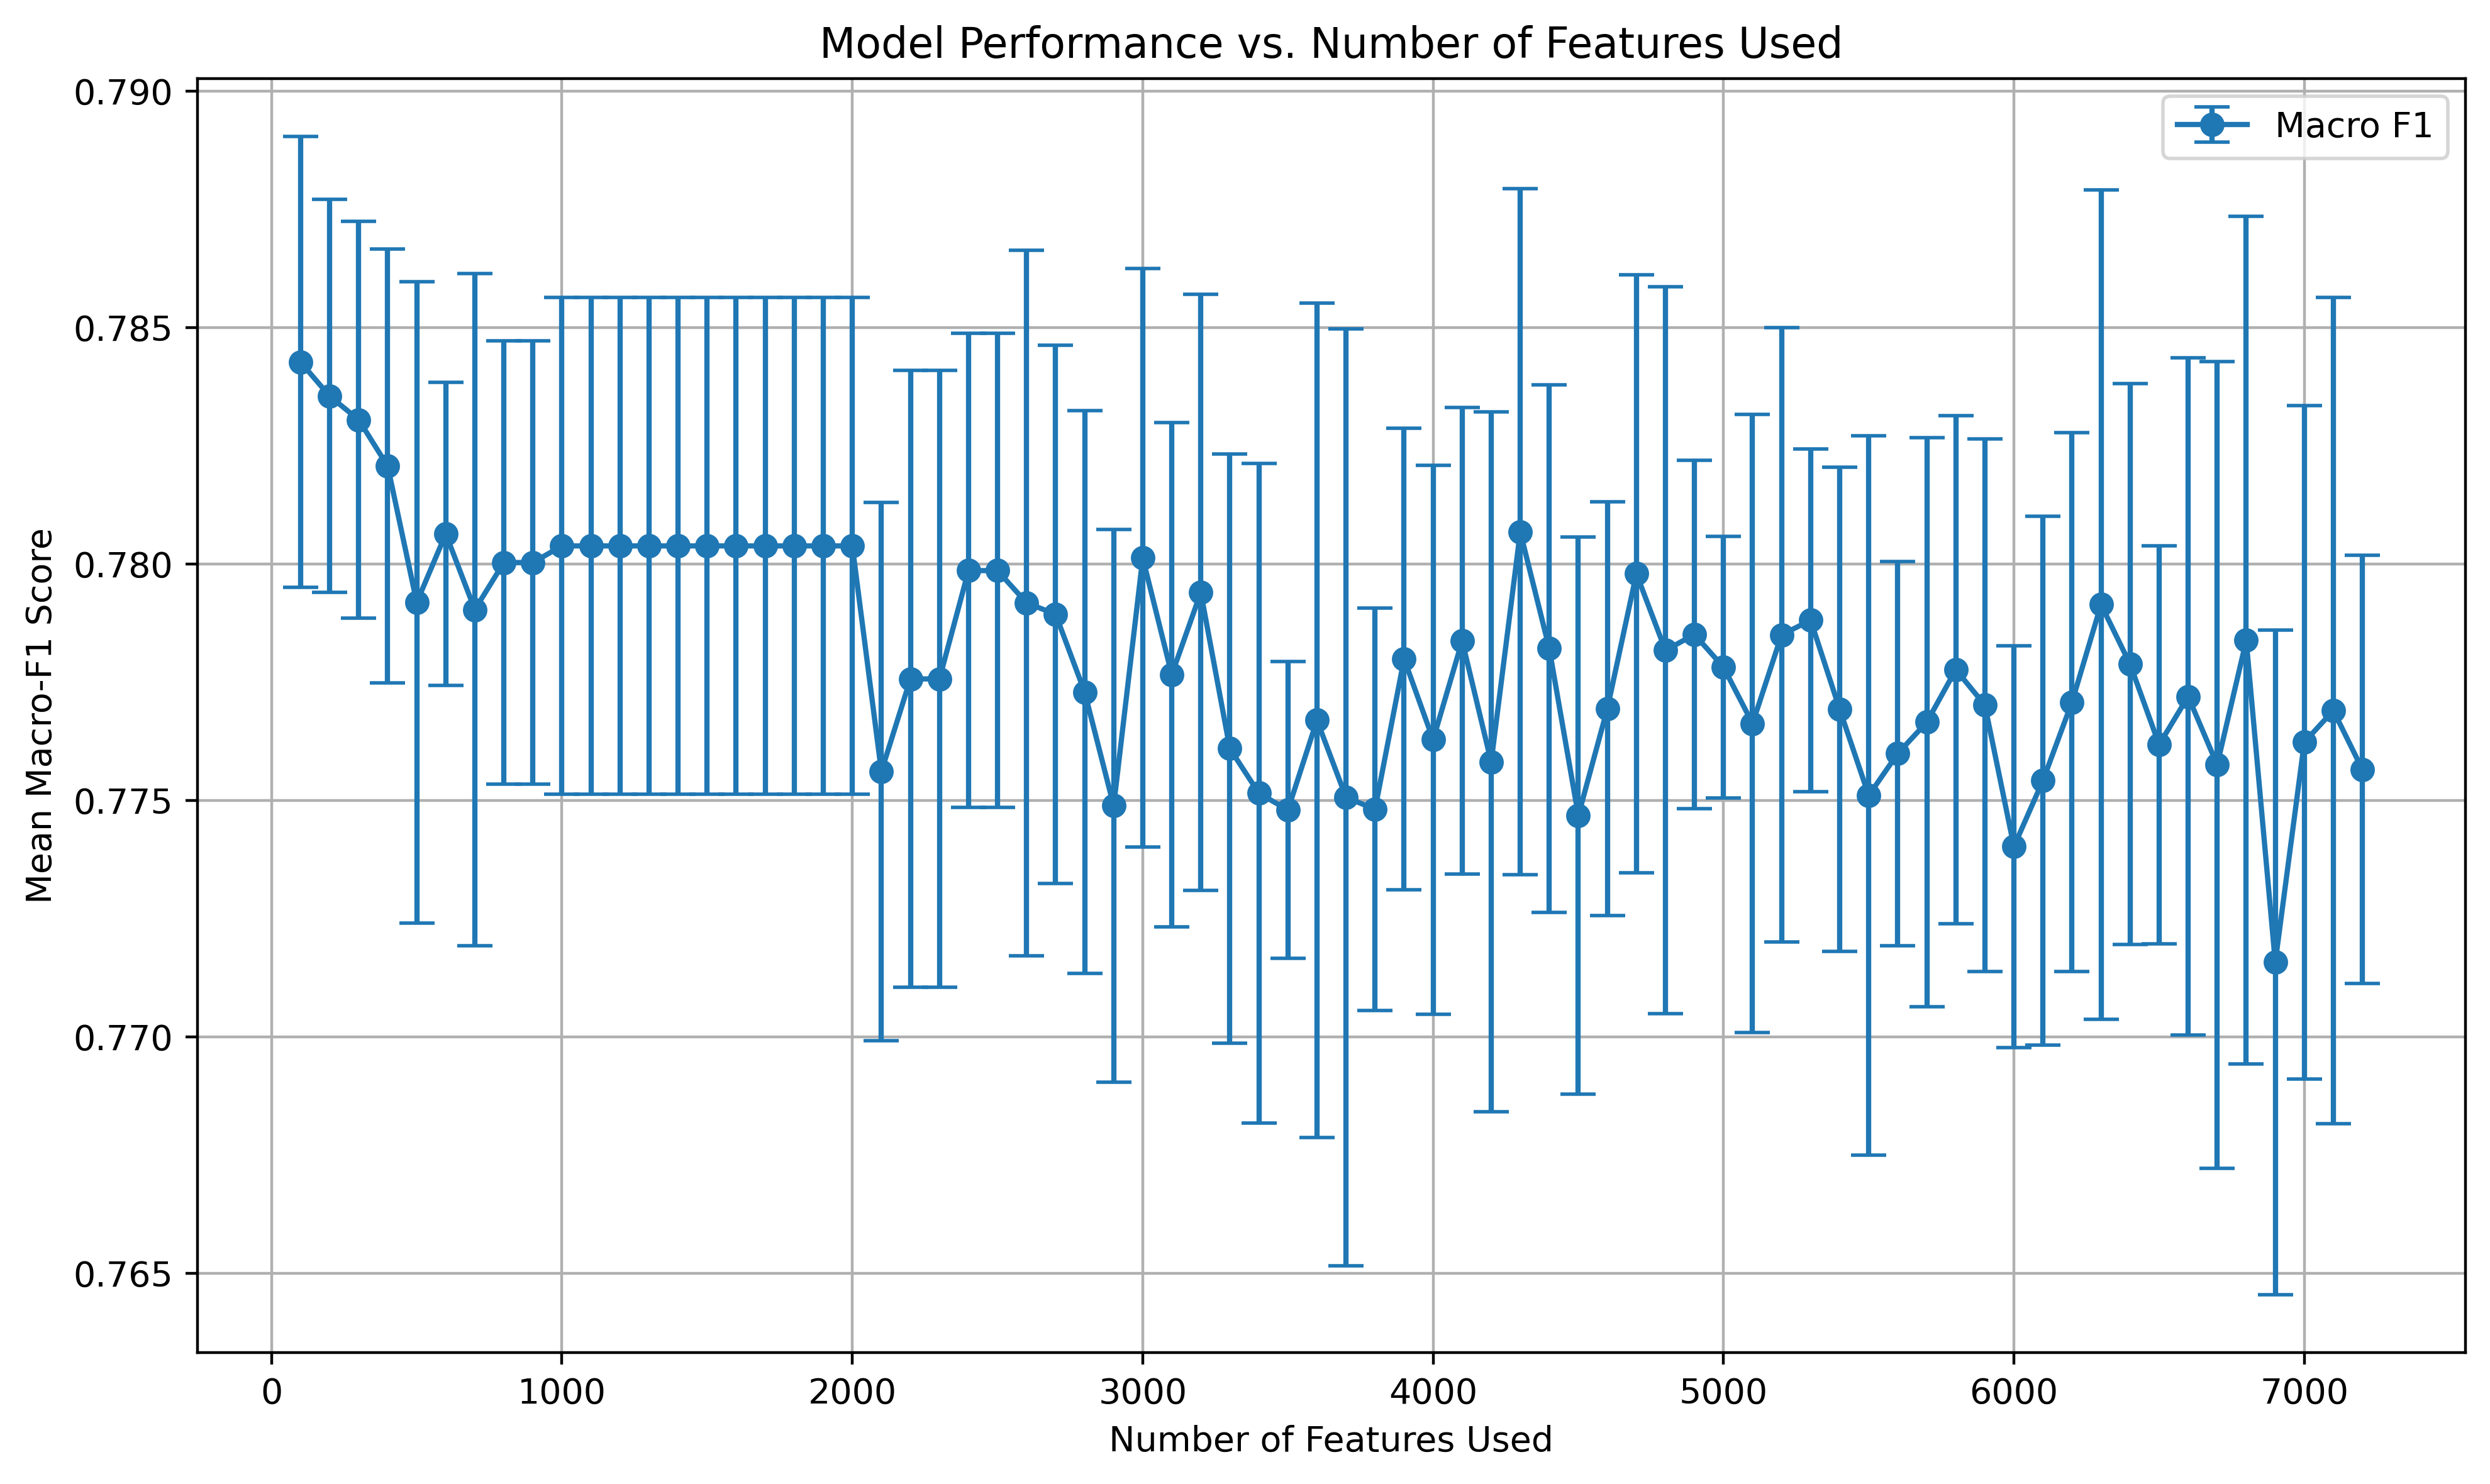
\includegraphics[width=\columnwidth]{../../results/images/model_n_feats.png}
    \caption{Performance of LGBM classifier vs number of features used by the classifier}
    \label{fig:features}
\end{figure}
Since embeddings appeared to be the most useful feature set, we trained the model on all the embeddings datasets we had computed to identify any noticeable difference. It resulted that the best performing embeddings are the mean pooled embeddings extracted from AlBERTo using Sentence Transformers.

With regard to the offensiveness score, we found that the score normalized by the length of the tweet yielded better results than both than the non-normalized score and the combination of the two scores.

Lastly, using the insights we had gained, we conducted a more comprehensive randomized search to re-tune the Light-GBM model's hyperparameters in order to have a definitive model to use for testing. The model reached an average F1-macro of 0.778 on the validation set. For the cross-domain task, given the significant stylistics differences between tweets and newspaper headlines, we decided to perform a second tuning to train another model excluding stylistic features.
